\chapter{Approach}\label{chap:approach}
To semantically segment urban scenes and extract predictions for curbs and curb cuts, we proposed to use a deep neural network based on the DeepLab v3+ architecture with a loss function inspired by "U-Net: Convolutional Networks for Biomedical Image Segmentation" by Olaf Ronneberger et al.~\cite{unet}.
In this chapter, the architecture used and an explanation of our loss function will be discussed.

\section{Architecture Selection} \label{section:approach-architectureselection}
We came to use the DeepLab v3+ architecture after running these experiments due to significantly outperforming the other networks. A further discussion of the results can be found in section \ref{section:experiments-networkevaluation}.

\subsection{Network Architecture}\label{section:approach-networkarchitecture}
We propose to apply the DeepLab v3+ architecture to our stated problem of curb and curb cut segmentation.
The architecture itself is given in \figref{fig:approach-network} with further descriptions in Tables \ref{tab:drn}-\ref{tab:decoder}\footnote{The full implementation written using the PyTorch framework can be found at \url{github.com/yvan674/CurbNet}}.

\begin{figure}
	\centering
	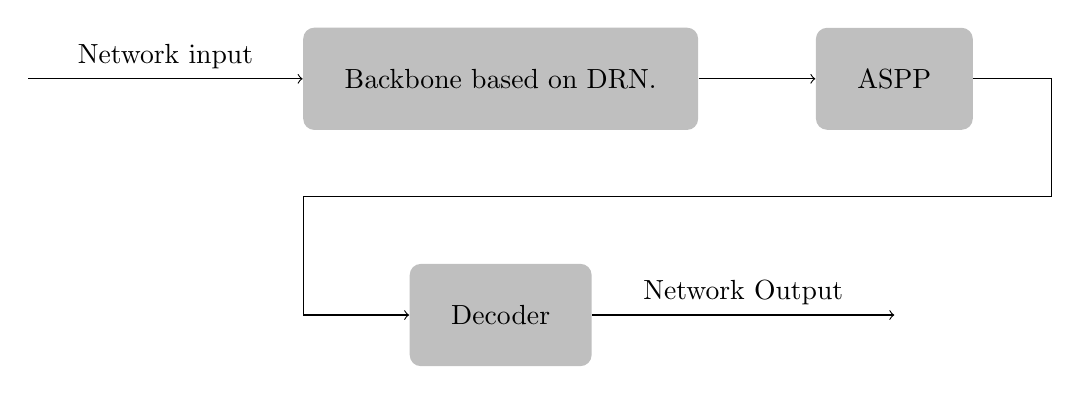
\begin{tikzpicture}
		% Backbone
		\node[fill=lightgray,rounded corners,inner sep=15pt] (backbone) at (0,0) {Backbone based on DRN.};
		% ASPP
		\node[fill=lightgray,rounded corners,inner sep=15pt] (ASPP) at (5,0) {ASPP};
		% Decoder
		\node[fill=lightgray,rounded corners,inner sep=15pt] (Decoder) at (0,-3) {Decoder};
		
		% Input arrow
		\draw [->] ++(-6,0) -- (backbone)
		node [above, midway] {Network input};
		% Backbone to aspp
		\draw [->] (backbone) -- (ASPP);
		% aspp to decoder
		\draw [->] (ASPP) -- (7,0) -- (7,-1.5) -- (-2.5,-1.5) -- (-2.5, -3) -- (Decoder);
		% Ouput arrow
		\draw [->] (Decoder) -- (5, -3)
		node [above, midway] {Network Output};

	\end{tikzpicture}
	\caption[Simplified Network Architecture]{A simplified visualization of the network architecture. The contents of each module is listed in Tables \ref{tab:drn}-\ref{tab:decoder}.}\label{fig:approach-network}
\end{figure}

\begin{table}
	\resizebox{\textwidth}{!}{%
	\begin{tabular}{@{}clL@{}}
		\toprule
		Layer & Module & \text{Parameters} \\ \midrule
		0 & Convolution + ReLU & \text{in}=5,~\text{out}=16,~\text{kernel}=7,~\text{stride}=1 \\ \midrule
		1 & Convolution + ReLU & \text{in}=16,~\text{out}=16,~\text{kernel}=3,~\text{stride}=1 \\ \midrule
		2 & Convolution + ReLU & \text{in}=16,~\text{out}=32,~\text{kernel}=2,~\text{stride}=1 \\ \midrule
		\multirow{3}{*}{3} & Bottleneck & \text{in}=32,~\text{low}=64,~\text{out}=256 \\
		 & Bottleneck & \text{in}=256,~\text{low}=64,~\text{out}=256 \\
		 & Bottleneck & \text{in}=256,~\text{low}=64,~\text{out}=256 \\ \midrule
		\multirow{4}{*}{4} & Bottleneck & \text{in}=256,~\text{low}=128,~\text{out}=512 \\
		 & Bottleneck & \text{in}=512,~\text{low}=128,~\text{out}=512 \\
		 & Bottleneck & \text{in}=512,~\text{low}=128,~\text{out}=512 \\
		 & Bottleneck & \text{in}=512,~\text{low}=128,~\text{out}=512 \\ \midrule
		\multirow{6}{*}{5} & Bottleneck & \text{in}=512,~\text{low}=256,~\text{out}=1024 \\
		 & Bottleneck & \text{in}=1024,~\text{low}=256,~\text{out}=1024 \\
		 & Bottleneck & \text{in}=1024,~\text{low}=256,~\text{out}=1024 \\
		 & Bottleneck & \text{in}=1024,~\text{low}=256,~\text{out}=1024 \\
		 & Bottleneck & \text{in}=1024,~\text{low}=256,~\text{out}=1024 \\
		 & Bottleneck & \text{in}=1024,~\text{low}=256,~\text{out}=1024 \\ \midrule
		\multirow{3}{*}{6} & Bottleneck & \text{in}=1024,~\text{low}=512,~\text{out}=2048 \\
		 & Bottleneck & \text{in}=2048,~\text{low}=512,~\text{out}=2048 \\
		 & Bottleneck & \text{in}=2048,~\text{low}=512,~\text{out}=2048 \\ \midrule
		7 & Convolution + ReLU & \text{in}=2048,~\text{out}=512,~\text{kernel}=3,~\text{stride}=1 \\ \midrule
		8 & Convolution + ReLU & \text{in}=512,~\text{out}=512,~\text{kernel}=3,~\text{stride}=1  \\ \bottomrule
	\end{tabular}
	}
	\caption{Dilated Residual Network Module Details}
	\label{tab:drn}
\end{table}
\begin{table}
	\resizebox{\textwidth}{!}{%
	\begin{tabular}{@{}clL@{}}
		\toprule
		Layer & Module & \text{Parameters} \\ \midrule
		0 & Convolution & \text{in}=\text{in},~\text{out}=\text{low},~\text{kernel}=1,~\text{stride}=1 \\ \midrule
		1 & Convolution & \text{in}=\text{low},~\text{out}=\text{low},~\text{kernel}=3,~\text{stride}=1 \\ \midrule
		2 & Convolution + ReLU & \text{in}=\text{low},~\text{out}=\text{out},~\text{kernel}=1,~\text{stride}=1 \\ \bottomrule
	\end{tabular}
	}
	\caption{Bottleneck Module Details}
	\label{tab:bottleneck}
\end{table}
\begin{table}
	\resizebox{\textwidth}{!}{%
	\begin{tabular}{@{}clL@{}}
		\toprule
		Layer & Module & \text{Parameters} \\ \midrule
		0 & Convolution + ReLU & \text{in}=512,~\text{out}=256,~\text{kernel}=1,~\text{stride}=1 \\ \midrule
		1 & Convolution + ReLU & \text{in}=512,~\text{out}=256,~\text{kernel}=1,~\text{stride}=1 \\ \midrule
		2 & Convolution + ReLU & \text{in}=512,~\text{out}=256,~\text{kernel}=1,~\text{stride}=1 \\ \midrule
		3 & Convolution + ReLU & \text{in}=512,~\text{out}=256,~\text{kernel}=1,~\text{stride}=1 \\ \midrule
		\multirow{2}{*}{4} & Global Average Pool & \text{in}=1280,~\text{out}=256 \\
		 & Dropout & p=0.5 \\ \bottomrule
	\end{tabular}
	}
	\caption{Atrous Spatial Pyramid Pooling (ASPP) Module Details}
	\label{tab:aspp}
\end{table}
\begin{table}
	\resizebox{\textwidth}{!}{%
	\begin{tabular}{@{}clL@{}}
		\toprule
		Layer & Module & \text{Parameters} \\ \midrule
		0 & Convolution + ReLU & \text{in}=256,~\text{out}=48,~\text{kernel}=1,~\text{stride}=1 \\ \midrule
		\multirow{2}{*}{1} & Convolution + ReLU & \text{in}=304,~\text{out}=256,~\text{kernel}=3,~\text{stride}=1 \\
		 & Dropout & p=0.5 \\ \midrule
		\multirow{2}{*}{2} & Convolution + ReLU & \text{in}=256,~\text{out}=256,~\text{kernel}=3,~\text{stride}=1 \\
		 & Dropout & p=0.5\\ \midrule
		3 & Convolution & \text{in}=256,~\text{out}=3,~\text{kernel}=1,~\text{stride}=1 \\ \bottomrule
	\end{tabular}
	}
	\caption{Decoder Module Details}
	\label{tab:decoder}
\end{table}

\section{Loss Function}\label{section:approach-lossfunction}
We chose to use a modified weighted cross entropy loss due to the severe class imbalance.
Using the assumption that all curbs and curb cuts must be located along the perimeter of roads, we used a loss function inspired by the paper "U-Net: Convolutional Networks for Biomedical Image Segmentation," which we call Masked Cross Entropy (MCE) and defined in \eqref{eq:mce}~\cite{unet}.
The weighted cross entropy loss function was modified to penalize according to the given weights when labeling within a certain border around road classes, which we call the mask $M$.
We define road classes $\text{class}_{\text{road}}$ as all classes which can reasonably be expected to be found on roads, including road, road markings, potholes, etc.
This mask was calculated using a binary dilation on a full $b \times b$ matrix $B$ where $b$ is $0.05 \times \text{image}_{width}$ on the road class, then subtracted by the road class itself.
Thus, this can be formalized as follows:
\begin{align}
	B &= \underbrace{
			\begin{bmatrix}
				1  & \cdots & 1\\ 
				\vdots &  \ddots & \vdots\\ 
				1 &  \cdots & 1
				\end{bmatrix}}_{b \text{ columns and } b \text{ rows}} \\
	M &= \left(\text{class}_{\text{road}} \oplus B\right) - \text{class}_{\text{road}}
\end{align}
A visualization of this mask applied to a color street-level image from the Mapillary dataset results in Figure \ref{fig:approach-mask}.
\begin{figure}
	\centering
	\includegraphics[width=0.7\textwidth]{figures/approach/mask/image/mask.jpg} % first figure itself
	\caption[Masked Cross Entropy Mask]{An example of the resulting mask that is used by masked cross entropy loss. The areas in the image that are marked with a blue overlay are the areas contained within the mask. The street-level color image was taken from the Mapillary dataset \cite{mapillary}} \label{fig:approach-mask}

\end{figure}

The value 0.05 was chosen empirically after looking at samples in the dataset and measuring what area around roads are typically curbs.
The road class was simply taken from the ground truth data.
Any labeling outside of $M$ by the network are then given an increased penalty, incentivizing the network to focus labeling around road edges.
We chose to multiply the penalty for areas outside $M$ by a factor of 3.
This can be seen in the following formalization of the loss function we used:
\begin{align}\label{eq:mce}
	\ell_{MCE}(y, \hat{y}) &=\sum_{m}-y_m\log(\hat{y}_m) \cdot d_m\\
	\text{with } d_m &= 
	\begin{cases}
	d_m' & \text{if } x \in M\\
	d_m' \cdot 3 & \text{if } x \notin M
	\end{cases}
\end{align}
where $d_m'$ are the user defined weights. 
This loss function operates on the assumption that curbs and curb cuts must be located adjacent to roads.
A visualization of the resulting mask $M$ can be seen in Figure \ref{fig:approach-mask}.
